%% CONDENSED version of "Budget-fair attribution of the gains of learning-guided Iterated Greedy" (the full manuscript with every table, battery and proof is journal/main.tex, the supplementary material).
%% Build: bash journal/build_short.sh   (pdflatex -> bibtex -> pdflatex x2). Numbers are checked by analysis/audit_journal_short.py against the audited full manuscript.
\documentclass[preprint,12pt,authoryear]{elsarticle}

\usepackage[utf8]{inputenc}
\usepackage[T1]{fontenc}
\usepackage{amsmath,amssymb,amsfonts,amsthm}
\usepackage{graphicx}
\usepackage{booktabs}
\usepackage{multirow}
\usepackage{longtable}
\usepackage{url}
\usepackage{xcolor}
\usepackage{setspace}
\usepackage{enumitem}
\setlist{nosep,topsep=2pt,itemsep=1pt,parsep=0pt,leftmargin=*}
\graphicspath{{../cec/}{./}}
\newif\ifdraftmarks \draftmarkstrue
\newcommand{\todonote}[1]{\ifdraftmarks\textcolor{red}{\textbf{[#1]}}\fi}
\newcommand{\Cmax}{C_{\max}}
\let\cite\citep
% counters of the registry (the same as main.tex; audited by analysis/audit_journal_claims.py)
\newcommand{\npredheld}{363}\newcommand{\npredtotal}{465}\newcommand{\nbatteries}{65}\newcommand{\npredshare}{78}
\newtheorem{proposition}{Proposition}
\hyphenation{learn-heu-ris-tics}
\sloppy

\journal{(journal to be chosen)}

\begin{document}
\begin{frontmatter}

\title{Budget-fair attribution of the gains of learning-guided metaheuristics: where does online learning pay?}

\author{Carlos Vin\'icio Dantas Ara\'ujo\corref{cor1}}
\ead{carlos.vinicio@aluno.uece.br}
\address{Graduate Program in Computer Science, State University of Cear\'a (UECE), Fortaleza, Brazil}
\cortext[cor1]{Corresponding author.}
\todonote{advisor/coauthor, funding statement and the anonymised repository link are the author's to add}

\begin{abstract}
Learning-guided metaheuristics are routinely reported to beat their non-learning counterparts, yet comparisons seldom separate what the learned policy adds from what the search structure, the CPU budget and the tuning already provide. We propose a budget-fair attribution protocol (a random control at a matched budget; equal CPU time, with the gain split into a decision effect and a cost effect; a static action validated offline; a cross-fitted oracle headroom; equivalence margins; hypotheses recorded before each run) and apply it, at $10^3$--$10^4$ iterations, to Iterated Greedy for scheduling, a permutation flowshop, a genetic algorithm, a TSP local search and, with the selectors of a third-party library, an adaptive large neighbourhood search for vehicle routing, in \nbatteries{} batteries. (1) Structure and budget explain much of what is credited to learning: destruction--reconstruction, not the policy, explains the IG's advantage over an iterated local search, and the share of a local search's gain that is only budget depends on the implementation ($28$--$93\%$). (2) A learner's gain can measure the order of its action list: the standard Q-Learning repeats the action listed first; breaking ties at random removes the lock-in and leaves a modest learner (beyond the equivalence margin in $32$ of $85$ cells, $12$--$18\%$ of the validated gain on the standard benchmark, following the headroom), whereas permuting the list once per run, our first control, is not a valid control. (3) A static action validated offline was almost never beaten at equal iterations ($2$ of $85$ cells by the random-tie learner; $2$ of $49$ pairs at equal CPU time), but this compares information, not learning: its tuning costs $11$ times its test run, one tuning instance per class gives $81\%$ of its gain, and with the tuning charged random choice with the same total compute does better for classes of fewer than about $72$ to $130$ instances. A warm-started online learner corrects a transferred prior ($+0.67$ points) but not a merely noisy one: even with one tuning instance per class it does not beat the static action, though it is half as sensitive to that sample. With heterogeneous operators the best of five library selectors recovers $23$--$61\%$ of the validated gain (one bandit loses) and is level with the best offline action on published instances unlike the tuning classes. Three domains; registrations kept in a private, hash-stamped diary.

\end{abstract}

\begin{keyword}
learnheuristics \sep adaptive operator selection \sep iterated greedy \sep parallel machine scheduling \sep experimental methodology \sep reinforcement learning
\end{keyword}
\end{frontmatter}

\onehalfspacing
\section{Introduction}
\label{sec:intro}
Metaheuristics that learn while they search are a prominent line of work in evolutionary computation and operations research. A typical \emph{learnheuristic}~\cite{CalvetEtal2017} embeds a reinforcement-learning agent, most often tabular Q-Learning~\cite{WatkinsDayan1992,SuttonBarto2018}, as an adaptive selector of operators, strategies or parameters inside a search framework such as Iterated Local Search (ILS)~\cite{LourencaoEtal2019} or Iterated Greedy (IG)~\cite{RuizStutzle2007}. The usual evidence is a comparison with the search without the agent, or with published baselines~\cite{KarimiMamaghanEtal2023,MissaouiOSullivan2026}; when the learned version wins, the result is read as evidence that the \emph{learned policy} is what helps.

That reading is fragile for three reasons. First, the \emph{search structure} that hosts the agent (its operators, its acceptance rule, its local search) may produce most of the gain under any selection rule. Second, the \emph{budget}: an agent changes the CPU time per iteration, so equal iteration counts are not equal budgets, and a policy that merely chooses cheaper actions buys extra iterations without having decided anything better. Third, the \emph{tuning}: a parameter validated offline on separate instances is a competitor that most studies omit, although a practitioner would use it before reaching for a learner. Adaptive operator selection (AOS) is well studied~\cite{FialhoEtal2010,PisingerRopke2007}, but in an audit of $23$ recent open-access papers that embed a learned selector in a metaheuristic, $10$ include a random-selection control, $6$ compare at a common time limit, $3$ include a static configuration tuned offline, and $22$ report a benefit of the learned component ($5$ of them only partly). The audit is small and has a single coder; its coding sheet is in the repository.

\paragraph{Research questions} \textbf{RQ1:} what explains the advantage of a learning-guided IG over ILS, and how much of a local search's gain is only budget? \textbf{RQ2:} do online learners beat random choice over the same actions, at equal iterations and at equal CPU time; does a static configuration win anyway; and could learning have shown up if it existed? \textbf{RQ3:} where, if anywhere, does an online selector pay, can that be foretold, and what exploits the headroom instead?

\paragraph{Contributions} (i) A \emph{budget-fair attribution protocol} (Section~\ref{sec:protocol}): a random control at a matched budget, a split of a learner's gain at equal CPU time into a decision effect and a cost effect, a static competitor validated offline, a cross-fitted oracle headroom with a formal treatment of its bias, power checks, positive controls, an order-sensitivity check, a map of the offline knowledge given to the static competitor, and predictions recorded with code hashes before every battery; the protocol is released as a small library. (ii) Evidence from $\nbatteries$ pre-specified batteries on six hosts (identical parallel machines, unrelated machines, a permutation flowshop, a genetic algorithm and, outside scheduling, an iterated local search for the travelling salesman problem and an adaptive large neighbourhood search for vehicle routing built on a third-party library) that the advantage of the learning-guided IG comes from its search structure and that the standard Q-Learning wins at equal CPU time by choosing cheaper actions, not by a learned policy. (iii) A \emph{headroom analysis}: the usual one-seed oracle headroom is mostly run-to-run noise; with the noise removed it is a necessary condition for a Q-Learning that does not lock in to pay (rank correlation $0.81$ across $28$ classes), never shown sufficient, and a policy learned \emph{offline} exploits it. (iv) A \emph{map of offline knowledge} and the finding that an online learner is best used as a \emph{corrector} of offline knowledge: warm-started with an offline prior it adds value where the prior was transferred and costs where it was exact, on a scheduling benchmark and, against a deliberately wrong prior, on the TSP. (v) A candid account of two reversals: the standard Q-Learning seemed to recover half to two thirds of the validated action's gain on published instances, but it repeats the action listed first; and our first order-invariant control, a permutation of the action list once per run, gains in none of $85$ cells but is itself a lock-in learner: with ties broken at random the learner gains beyond the margin in $32$ of the $85$ cells, in step with the headroom, and recovers $12$--$18\%$ of the validated gain on the standard benchmark. (vi) The price of offline knowledge: tuning a validated action costs $11$ times its test run, one tuning instance per class gives $81\%$ of its gain, and with the tuning charged its advantage over random choice depends on how many instances each class will see.

\paragraph{Outline} Section~\ref{sec:related} places the work among parameter control, algorithm selection and configuration, and benchmarking methodology. Section~\ref{sec:method} describes the hosts, learners and protocol. Section~\ref{sec:results} answers the research questions and reports the order diagnostic. Section~\ref{sec:external} tests how far the answers carry: published instances, equal CPU time, a longer horizon, offline policies, the value of offline knowledge and a second domain. Section~\ref{sec:discussion} discusses when online learning pays, gives a checklist and lists the limitations. This is the condensed version of the full manuscript, whose supplementary sections hold every table, battery and proof (the numbers here are checked against them by an audit script).

\section{Related work}
\label{sec:related}
\paragraph{Parameter control, hyper-heuristics and learning inside metaheuristics} Choosing among operators during a run is the subject of parameter control~\cite{EibenEtal1999,KarafotiasEtal2015} and of selection hyper-heuristics~\cite{BurkeEtal2013,DrakeEtal2020}. Adaptive operator selection~\cite{FialhoEtal2010} combines a credit-assignment rule with a selection rule: probability matching~\cite{Goldberg1990}, adaptive pursuit~\cite{Thierens2005}, ALNS-style weights~\cite{PisingerRopke2007}, bandits~\cite{AuerEtal2002,DaCostaEtal2008} or reinforcement learning with a state~\cite{BengioBengio2021}; we include all of them as learners. Q-Learning has been used to select operators inside an IG for the permutation flowshop~\cite{KarimiMamaghanEtal2023} and the destruction size of an IG for identical machines with setups~\cite{MissaouiOSullivan2026}; both report that the learning-guided method beats its baselines. Where learned neighbourhood selection beats strong baselines on routing problems the policy is trained offline across instances~\cite{SonneratEtal2021}, as is dynamic algorithm configuration~\cite{BiedenkappEtal2020,EimerEtal2021}, whose tabular form we test.

\paragraph{Offline configuration, algorithm selection and the oracle} Configurators such as irace~\cite{LopezIbanezEtal2016} and ParamILS~\cite{HutterEtal2009} fix the parameters before the run, and tuning and control are two ways of configuring the same algorithm~\cite{EibenSmit2011}; the validated static action and the irace-configured algorithm are therefore the natural competitors of an online learner. In algorithm selection~\cite{Rice1976,KerschkeEtal2019,BischlEtal2016} a selector is scored by the share of the gap between the single best solver and the per-instance oracle that it closes. Our one-seed oracle is that oracle, relative to random choice; what is specific here is that the oracle of a \emph{stochastic} algorithm is inflated by run-to-run noise (a winner's curse), which we remove by cross-fitting~\cite{ChernozhukovEtal2018}.

\paragraph{Benchmarking methodology and what is new} The literature has long asked for controlled experiments with hypotheses stated beforehand~\cite{Hooker1995,BarrEtal1995,LaTorreEtal2021,BartzBeielsteinEtal2020}, and reinforcement-learning research has documented how sensitive reported gains are to seeds and implementations~\cite{Henderson2018}. We follow that spirit with equivalence tests~\cite{Lakens2017} and preregistration~\cite{NosekEtal2018}. Each ingredient is established practice in some community; the contribution is their combination for adaptive selectors, the decision/cost decomposition, the cross-fitted headroom as a necessary-condition diagnostic, and the evidence assembled with them, plus two diagnostics absent from the controls coded in our audit: the sensitivity of a learner to the order of its actions and the value of the offline knowledge given to the static competitor.

\section{Method}
\label{sec:method}
\subsection{Problems, instances and hosts}
\label{sec:instances}
In $P||\Cmax$, $n$ jobs with processing times $p_j$ are assigned to $m$ identical machines to minimise $\Cmax=\max_i\sum_{j\in S_i}p_j$; the classical bound is $\mathrm{LB}=\max(\max_jp_j,\lceil\sum_jp_j/m\rceil)$~\cite{Graham1969}. The \emph{synthetic} instances have $p_j\sim U[1,100]$ in twelve classes $(n,m)$ from $(20,4)$ to $(300,20)$, with $100$ test and $30$ separate tuning instances per class; the \emph{published} families B, C, E and F of the benchmark reviewed by \citet{OstojicEtAl2025} give disjoint sets of $525$ tuning, $2{,}550$ discovery and $3{,}950$ held-out test instances, $5{,}720$ instances on which an offline selector is trained, and $780$ of family F. In $R||\Cmax$ the time $p_{jk}$ depends on the machine: we use (a) the twelve synthetic classes with $p_{jk}\sim U[1,100]$, (b) three published families (uncorrelated, correlated jobs, correlated machines~\citep{AbladEtAl2021}; $25$ sizes each, generated by us from the description), and (c) the \emph{standard benchmark} of Fanjul-Peyro and Ruiz~\citep{FanjulPeyroRuiz2010}: $1{,}400$ instances of seven types with $m\in\{10,\dots,50\}$ and $n\in\{100,\dots,1000\}$, with best known values from CPLEX, Gurobi and an exact Lagrangian method run by third parties (the minimum of the three is proven optimal for $73\%$ of the test instances); two instances per cell tune and five test ($280$ tuning and $700$ test instances). The other hosts are a permutation flowshop (nine synthetic classes and the $90$ instances of \citet{Taillard1993}), a steady-state genetic algorithm for $P||\Cmax$ ($1{,}200$ instances) and, outside scheduling, an iterated local search for the Euclidean TSP on generated instances and on $37$ instances of the TSPLIB (Section~\ref{sec:tsp}).

\subsection{Search mechanisms and learners}
\label{sec:learners}
The \textbf{IG} starts from LPT and alternates destruction (removing $d$ jobs) and greedy reconstruction, accepting a candidate that does not worsen the makespan. The \textbf{ILS} chooses at each iteration one of four neighbourhood operators. The \emph{actions} of the IG are the destruction strategy ($3$), the destruction size ($5$), their $15$ combinations and these with or without a descent after reconstruction ($30$); on the standard benchmark the sizes scale with $n$ (B5, B15, B30). At each iteration a selector chooses an action from a state of $81$ values (gap to the bound, load imbalance, fraction of the budget used, stagnation), receives as reward the improvement of the makespan truncated at zero, and the selector is the only component that changes between arms. The learners are tabular Q-Learning ($\alpha=0.1$, $\gamma=0.9$, $\varepsilon$ from $1.0$ to $0.05$)~\cite{WatkinsDayan1992}, UCB1~\cite{AuerEtal2002}, a policy gradient~\cite{Williams1992}, six stateless methods (probability matching, adaptive pursuit, an ALNS roulette, discounted Thompson sampling~\cite{Russo2018}, DMAB~\cite{DaCostaEtal2008}, online racing), LinUCB~\cite{LiEtAl2010}, a DQN~\cite{MnihEtAl2015}, an optimistic Q-Learning (optimistic table of initial value $c$, constant $\varepsilon=0.05$, scale-invariant reward) and two re-implemented published designs (an episodic Q-Learning in the style of \citet{KarimiMamaghanEtal2023} and an FRRMAB-style bandit~\cite{LiFialhoEtal2014}); hyperparameters are tuned on tuning instances and then frozen. \emph{Random choice} over the same actions is the control; the \emph{static competitor} is the best fixed action per class on the tuning instances.

\paragraph{Action order and ties} The standard Q-Learning starts from a table of zeros, its reward is non-negative and its greedy step takes the \emph{first} maximum; in an unvisited state all values are equal, so after the exploration rate has decayed it repeats the action with the smallest index (the smallest and cheapest, as our lists are ordered by size). We therefore report the standard implementation (\textsc{ql}) and an order-invariant version (\textsc{ql-perm}) that permutes the actions at random in each run, which is equivalent to breaking ties at random.

\subsection{The budget-fair attribution protocol}
\label{sec:protocol}
A \emph{class} is an $(n,m)$ pair or a published family by size tercile; a \emph{cell} is a class in one action space; the \emph{validated action} is the best fixed action per class, chosen on separate instances; the \emph{headroom} of a cell is the gain over random choice of the best fixed action per instance. A \emph{gain} is $-\bar d$ in percentage points of the makespan, positive when the first-named arm is better; \emph{registered} results were specified before the battery was run, \emph{post hoc} ones were not.
\begin{enumerate}
\item \textbf{Random control at a matched budget.} The effect of the policy is the difference between the learner and uniform random choice over the same actions, iterations and instances.
\item \textbf{Equal CPU time and the decision/cost split.} The ratio $K$ of the CPU time of $1000$ iterations of one arm to that of another is measured on separate instances and the second arm receives $\mathrm{round}(1000K)$ iterations. With $\bar d_{\mathrm{iter}}$ and $\bar d_{\mathrm{CPU}}$ the mean relative differences of the learner against random choice at equal iterations and at equal CPU time,
\begin{equation}
G_{\mathrm{CPU}}=G_{\mathrm{dec}}+G_{\mathrm{cost}},\qquad G_{\mathrm{dec}}=-\bar d_{\mathrm{iter}},\qquad G_{\mathrm{cost}}=\bar d_{\mathrm{iter}}-\bar d_{\mathrm{CPU}}.
\label{eq:decomp}
\end{equation}
A learner with $G_{\mathrm{dec}}\le0$ and $G_{\mathrm{cost}}>0$ wins at equal CPU time without having decided anything better.
\item \textbf{A static competitor validated offline}: the best fixed action per class and, when actions are complementary, a uniform mixture of the best few; at equal CPU time it receives its own cost ratio.
\item \textbf{Cross-fitted oracle headroom.} The action is chosen on two seeds and evaluated on two fresh ones (Section~\ref{sec:estimator}).
\item \textbf{Power and positive controls}: the minimum detectable gain, analytic and by planting gains in the paired differences, and a planted reward bonus.
\item \textbf{Order sensitivity}: the share of choices on the action listed first, and the learner with the actions permuted at random (Section~\ref{sec:order}).
\item \textbf{What the static competitor knows}: static policies chosen with decreasing knowledge of the instance (one action for all, one per size, per type, per class), in transfer regimes (the tested type or size withheld), compared with the learner and with the learner warm-started with the same knowledge (Section~\ref{sec:granularity}).
\end{enumerate}

\subsection{The cross-fitted headroom estimator}
\label{sec:estimator}
Let $Y_a(x)$ be the relative makespan of one run of action $a$ on instance $x$, with mean $\mu_a(x)$ and independent noise of variance $\sigma^2$; the headroom is $H(x)=\mu_{\mathrm{rand}}(x)-\min_a\mu_a(x)$. The \emph{one-seed oracle} $\hat H_1=\mu_{\mathrm{rand}}-\min_aY_a$ takes the best of one run per action; the \emph{cross-fitted oracle} chooses $\hat a=\arg\min_a\bar Y_a^{(1)}$ on two runs and evaluates it on two independent ones, $\hat H_{\mathrm{cf}}=\mu_{\mathrm{rand}}-\bar Y_{\hat a}^{(2)}$.
\begin{proposition}
\label{prop:bounds}
For every $x$, $\mathbb E[\hat H_{\mathrm{cf}}(x)]\le H(x)\le\mathbb E[\hat H_1(x)]$. If all $\mu_a(x)$ are equal, $\mathbb E[\hat H_{\mathrm{cf}}]=H=0$ and $\mathbb E[\hat H_1]\approx\sigma\sqrt{2\ln A}$ under normal noise.
\end{proposition}
The expectation of a minimum does not exceed the minimum of the expectations, so the one-seed value is an upper bound; conditional on $\hat a$, which depends only on the first batch, the second batch is unbiased for $\mu_{\hat a}\ge\min_a\mu_a$, so the cross-fitted value is a lower bound (proof and Monte Carlo check in the supplementary material). Every headroom statement below uses the cross-fitted value.

\subsection{Statistics, registration and reproducibility}
\label{sec:stats}
Per instance (the mean of the seeds), $d=100(A-B)/B$ is tested in pairs (Wilcoxon, two-sided), with Holm correction over each family, a bootstrap $90\%$ interval and an equivalence margin of $\pm0.05\%$~\cite{Lakens2017}: a Holm-significant difference whose interval lies inside the margin is \emph{parity}, and one whose interval crosses it a \emph{small win}; ``beyond the margin'' means confirmed and not equivalent to zero. The registered tests are pooled under a global Benjamini--Yekutieli control (Section~\ref{sec:discussion}). Hypotheses, decision rules and probabilistic predictions were written, with md5 hashes of the code and of the frozen inputs, in a dated, version-controlled research diary before each battery was run~\cite{NosekEtal2018}; each analysis script prints whether each prediction held. The code is compiled (numba) and covered by $1{,}577$ unit tests, and audit scripts recompute every number quoted in the text from the result files; all runs used one laptop (8 cores), where $K$ was measured.

\section{Results}
\label{sec:results}
Table~\ref{tab:answers} summarises the answers, separating registered findings from post hoc readings; the subsections give the evidence, and Section~\ref{sec:external} tests how far it carries.

\begin{table}[t]
\caption{Answers to the three research questions and the check on other hosts (gains in percentage points of the makespan).}
\label{tab:answers}
\centering
{\scriptsize\setlength{\tabcolsep}{3pt}
\begin{tabular}{@{}lp{7.6cm}p{2.6cm}l@{}}
\toprule
 & Answer & Status & Evidence \\
\midrule
RQ1 & Search structure, not the policy (the IG beats the ILS by $0.46\%$ at equal CPU time); budget is $93\%$, $30\%$ or $28\%$ of a local search's gain, by implementation & registered & \ref{sec:rq1} \\
RQ2 & On the synthetic classes no learner beats random choice at equal iterations by more than $0.04$ points; equal-CPU wins are cost effects; a validated action wins & registered & \ref{sec:rq2} \\
RQ3 & Headroom is a necessary condition only; an order-invariant Q-Learning gains in none of the $85$ cells where we repeated it; a selector trained offline captures the headroom (parity with the validated action; a neural policy, two thirds of its gain), no online repair works; one action for all instances beats every online learner on the standard benchmark, and an online learner beat an offline action only when it was transferred to an unseen size (post hoc), where warm-starting it with the offline prior adds $0.67$ points to the prior alone & registered (held-out test, cross-fitting); the rule and its one-sided reading are exploratory & \ref{sec:rq3}, \ref{sec:order}, \ref{sec:granularity} \\
Hosts & No online learner gains on a flowshop; the findings repeat in the TSP, outside scheduling; on a genetic algorithm only Thompson sampling does, and a validated mixture is never worse; on unrelated machines the validated action beats every learner & registered & \ref{sec:hosts}, \ref{sec:external} \\
\bottomrule
\end{tabular}}
\end{table}

\subsection{RQ1: the search structure and the budget, not the policy}
\label{sec:rq1}
Against LPT and seven ILS variants in the twelve classes, the Q-Learning-guided IG is significantly better, after Holm correction, in $72$ of $96$ comparisons and never worse, yet its advantage over its four ablation siblings (random selection, UCB1 with and without state, Q-Learning without state) is negligible: $0.011\%$ ($90\%$ interval $0.003$ to $0.019$). With learning removed from both sides, the IG beats the ILS at equal iterations in $10$ of $12$ classes by $0.49\%$, against $0.53\%$ for the learned versions; with vectorised operators ($6.2$ times faster), the IG still beats the ILS by $0.46\%$ at equal CPU time ($p_{\mathrm{Holm}}<10^{-80}$), with a positive gain in all twelve classes.

\emph{Budget.} A short best-improvement descent after each reconstruction improves the IG by $0.150\%$ at equal iterations but costs CPU time, so the verdict at equal CPU depends on $K$, and $K$ on the implementation. With the loop-based descent ($K=9.6$) the advantage at equal CPU is $0.010\%$ ($93\%$ of the gain would have been budget); vectorising it cuts $K$ to $1.8$ and the advantage at equal CPU is $0.105\%$ ($30\%$ budget); compiling both arms gives $K=2.0$ and $0.115\%$ of the $0.159\%$ ($28\%$), a reading registered before the compiled run. The share of a local search's gain that is ``only budget'' ranges from $28\%$ to $93\%$ with the implementation, so a claim about it is a claim about an implementation.

\subsection{RQ2: do learners beat random choice, does a static configuration win, and could learning have shown up?}
\label{sec:rq2}
\emph{At an equal number of iterations none of the three original learners gains more than $0.016\%$ over random choice in any of the $12$ comparisons}, within the equivalence margin. \emph{At equal CPU time Q-Learning does win} in the two spaces of sizes, by $0.059\%$ and $0.049\%$, \emph{but only by choosing cheaper actions}: its decision effect is nil ($-0.003$ and $-0.004$ points) and its cost effect is $0.062$ and $0.053$, an effect that an order-invariant version does not have (Section~\ref{sec:order}). Among the classic AOS methods only the ALNS-style roulette gains ($0.039$ points at equal iterations with five sizes, inside the margin), and online racing is \emph{worse} than random choice ($-0.012$ and $-0.067$). The configuration validated per class is ahead of every one of nine methods by $0.053$--$0.147$ points in the spaces of $5$ and $15$ actions ($p_{\mathrm{Holm}}<10^{-57}$); where the actions differ in effect and cost (the four ILS operators), a DQN and LinUCB lose to the uniform mixture ($0.041\%$ and $0.066\%$).

\emph{Could learning have shown up?} With $1{,}200$ pairs the analytic minimum detectable gain at $80\%$ power is $0.006$--$0.014$ points; planting gains gives $58$--$99.8\%$ power at $0.02$ points and at least $97\%$ at $0.03$, while the largest gain of Q-Learning, UCB1 or the policy gradient is $0.016$: gains of $0.03$ points or more are excluded. The per-class validated action is detected at $0.092$ and $0.080$ points, and with a reward bonus planted on one action all six learners tested choose it at least $1.5$ times more often than uniform. Longer horizons do not rescue the learner: with five sizes and $T$ up to $100{,}000$ the learners stay within $0.006$ points of random choice while the one-seed oracle headroom falls from $0.125\%$ to $0.015\%$.

\emph{Stronger competitors.} irace~\cite{LopezIbanezEtal2016}, given the tuning cost of the validated action, reaches parity with it on P$||\Cmax$ (within $0.012$ points) and stays $0.15$ and $0.19$ points behind on R$||\Cmax$, never ahead beyond the margin even with ten times the budget; the best three-phase schedule of the sizes per class adds nothing at the class level; two state-dependent look-ahead policies that are given hundreds of times a learner's evaluations are beaten by the validated action in all eight cells ($0.04$--$1.58$ points); tuning Q-Learning's hyperparameters beats the default by $0.58$ and $0.63$ points on R$||\Cmax$, yet the validated action beats it in all four host--space pairs ($0.06$--$1.90$). Two published AOS designs reach at most $14\%$ of the validated action's gain on R$||\Cmax$.

\subsection{RQ3: where does an online selector pay, and what exploits the headroom?}
\label{sec:rq3}
\paragraph{The oracle headroom is mostly noise unless it is cross-fitted} Taken as the best of one seed per action, the headroom of the synthetic classes is $0.125$ and $0.122$ points (five and fifteen actions); cross-fitting removes half to two thirds of it ($0.063$ and $0.043$), $28$--$40\%$ of that of the published instances, and $80$--$90\%$ on the flowshop, where run-to-run noise is high.

\paragraph{A necessary condition, not a sufficient one} Across the cells of a space, the rank correlation between the cross-fitted headroom and the \emph{standard} Q-Learning's gain is $0.95$ and $0.97$ on the held-out published instances, and a single threshold $h^*=0.048$ points, chosen on $18$ discovery cells, classifies $78\%$ of the $60$ others correctly (balanced accuracy $0.80$; Fig.~\ref{fig:class}). The robust reading is one-sided and post hoc: below $h^*$ there are $71$ cells outside the discovery set and in none does Q-Learning gain beyond the margin; above it there are $79$ and it does in $29$. The order diagnostic below qualifies even this: with the order-invariant learner the correlation on the held-out cells is $-0.74$, so what survives is the negative half of the rule.

\begin{figure}[t]
\centering
\includegraphics[width=0.78\textwidth]{fig_cec6.pdf}
\caption{Cross-fitted oracle headroom against the gain of the \emph{standard} Q-Learning over random choice at equal iterations, per cell: synthetic class by action space (grey), published family by size tercile by space ($18$ discovery cells, hollow; $18$ held-out, filled), flowshop (crosses), genetic algorithm (triangles) and synthetic class with finer times (squares). Dotted: the threshold $h^*$. Unrelated-machines cells are off scale.}
\label{fig:class}
\end{figure}

\paragraph{What exploits the headroom: a policy learned offline} An ExtraTrees regressor trained on $5{,}720$ disjoint instances with scale-free features and no family label picks one action per instance. On the published instances it gains $0.024$--$0.044$ points over the validated action (parity, except in one cell), $0.08$--$0.095$ over Q-Learning and captures $0.79$--$0.84$ of the one-seed oracle headroom against $0.58$--$0.66$ for the validated action; a per-class lookup table learned on the same instances is level with it, so most of the gain is class-level knowledge. On unrelated machines it beats the best online learner by $0.72$ and $1.91$ points but captures $60\%$ and $73\%$ of the headroom, no more than the validated action. Four repairs of the online learner (tuning per family, plateau rewards, a pre-trained Q table, optimistic initialisation) do not change the order: the limit is the learning signal (bandit feedback), not the cold start, since the selector sees every action's outcome on every training instance.

\subsection{Other hosts: a flowshop, a genetic algorithm and unrelated machines}
\label{sec:hosts}
\emph{Flowshop.} The cross-fitted headroom is only $0.012$ and $0.025$ points; no online learner beats random choice and the validated action beats the five learners in all ten pairs. \emph{Genetic algorithm.} The actions are complementary, so a single validated action can lose to uniform random choice ($-0.057$ with nine actions); Thompson sampling gains $0.051$ and $0.047$, Q-Learning loses, and the competitor that wins is a validated \emph{mixture} (specified after the single action lost on this host): it gains $0.050$ and $0.144$. \emph{Unrelated machines.} Here the headroom is real ($1.5$ and $2.8$ points one-seed, $0.43$ and $1.60$ cross-fitted; the validated action gains $0.95$ and $2.08$), yet at equal iterations Q-Learning loses ($-1.06$ and $-0.48$), and only the optimistic Q-Learning ($+0.17$) and the ALNS roulette ($+0.15$) gain beyond the margin, at most $18\%$ and $7\%$ of the validated gain; at equal CPU time Q-Learning and the roulette gain through the cost effect, and the validated action, with its own cost ratio, still beats all five learners in all ten pairs ($0.94$--$2.17$).

\subsection{A caveat on the standard Q-Learning: it depends on the order of the actions}
\label{sec:order}
The standard Q-Learning behaved in ways that looked like learning but were not: it lost to random choice by up to $1.19$ points where the static choice gains most, gained up to $65\%$ of the validated gain on published families, and won at equal CPU time ``by choosing cheaper actions''. A registered diagnostic showed that it puts $55$--$73\%$ of its choices on the action listed first (random choice: $3$--$20\%$). Moving the validated action of each class to index $0$ lifts the standard learner to $81\%$, $81\%$ and $86\%$ of the validated gain in the three spaces: it recovers an average action wherever the list puts one. Repeating the cells with the order-invariant version (Table~\ref{tab:order_b}), it gains beyond the margin in none of the $85$ cells ($21$ of the standard benchmark, $6$ of the published $R||\Cmax$ families, $24$ of the synthetic $P||\Cmax$ battery, $18$ of the held-out published $P||\Cmax$ instances, $16$ of the TSP host); on the held-out instances of family C, where the standard learner gained $0.245$ and $0.149$ points, it loses $0.25$ and $0.12$. The cost effect has the same cause: the standard learner evaluates $0.44$--$0.46$ times as many solutions as random choice, the order-invariant one $0.99$--$1.01$ times.

% Auto-generated by analysis/make_table_journal.py
\begin{table}[t]
\caption{The order-invariant Q-Learning (ql\_perm: a random permutation of the actions in each run) against the standard one and the validated action: mean gain over random choice across the cells of each battery (points, positive = better) and number of cells with a gain beyond the equivalence margin. Synthetic P$||C_{\max}$: $12$ classes $\times$ spaces S5 and S15; published P$||C_{\max}$: families B, C, E $\times$ size tercile $\times$ spaces S5 and S15.}
\label{tab:order_b}
\centering
{\scriptsize\setlength{\tabcolsep}{4pt}
\begin{tabular}{@{}lrrrrr@{}}
\toprule
Battery & cells & ql & ql\_perm & val & cells with ql\_perm gain \\
\midrule
Standard benchmark (Fanjul-Peyro, Ruiz) & 21 & $-$0.25 & $-$0.30 & 1.60 & 0 \\
Published $R||C_{\max}$ families & 6 & 0.28 & $-$0.33 & 1.28 & 0 \\
Synthetic $P||C_{\max}$ & 24 & 0.00 & $-$0.06 & 0.09 & 0 \\
Published $P||C_{\max}$, held-out & 18 & 0.02 & $-$0.07 & 0.08 & 0 \\
\bottomrule
\end{tabular}}
\end{table}


This removes the strongest evidence for online learning that the study had, together with the positive half of the headroom rule. Four things follow: the earlier gains of ``Q-Learning'' describe the standard implementation; what survives of the rule of use is its negative half; the protocol needs a rule it did not have (report the learner's order sensitivity or break ties at random); and the optimistic Q-Learning, UCB1 and the other bandits, which do not repeat the first index, are the more reliable representatives of online learning.

\section{External validity: published instances, a longer horizon, offline knowledge and a second domain}
\label{sec:external}
The synthetic classes are the weakest point of any such study because the authors chose them. We therefore repeated the protocol on instances that others defined, and then asked how far the conclusions carry.

\subsection{Published families and the standard benchmark}
\label{sec:families}\label{sec:fanjul}
On three published families of $R||\Cmax$ ($500$ test instances per family and space; learners with frozen hyperparameters, only the validated action re-chosen) the cross-fitted headroom exceeds the threshold in all six cells ($0.52$ to $2.31$ points) and the validated action beats every learner in all $30$ pairs ($0.42$--$2.64$ points). But the standard Q-Learning gains beyond the margin in four of the six cells, up to $0.67$ and $0.83$ points with correlated machines ($53\%$ and $65\%$ of the validated gain). We first read this as the most favourable evidence for online learning that we found, and withdraw that reading in Section~\ref{sec:order}: an order-invariant Q-Learning loses to random choice in all six cells. An irace-configured static action is at parity with the validated one in every cell; an irace-tuned Q-Learning and two published designs gain up to $0.82$ and $0.54$ points, and the validated action beats the three in all $18$ comparisons.

On the standard benchmark ($28$ classes of type and $n$, the validated action chosen on $10$ tuning instances per class, learners frozen) the validated action gains beyond the margin in all $21$ cells ($0.14$ to $5.08$ points) and is better than every learner in all $147$ learner--cell pairs; its mean gap to the best known solutions of the $700$ test instances is $4.89\%$ in the richest space (B30), against $7.42\%$ for random choice. The standard Q-Learning gains in three of its $21$ cells, loses up to $1.19$ points, and does worst where the static choice matters most; the diagnostic of Section~\ref{sec:order} explains why: it puts $55\%$ of its choices on the first, cheapest action. Five of the seven registered predictions held.

\subsection{Equal CPU time, a longer horizon and a neural policy}
\label{sec:eqcpu}\label{sec:longT}\label{sec:neural}
\emph{Equal CPU time.} Measured $K$ is $0.74$ for the standard Q-Learning, $0.98$--$1.07$ for most learners and $1.97$ for the validated action, which therefore runs about half as many iterations. The standard Q-Learning's cost effect is $+0.44$ points, so at equal CPU it is level with random choice ($-0.03$; at equal iterations $-0.46$) and wins beyond the margin in two of seven types, those where the cheapest action it repeats happens to be good. The validated action, with half the iterations, still beats the learners in $44$ of the $49$ learner--type pairs; two pairs go the other way (an outcome we had predicted not to happen), on correlated machines, where the local-search action is the most expensive (median $K=2.50$): the ALNS roulette and the FRRMAB-style design beat it by $0.29$ and $0.53$ points.

\emph{A ten times longer horizon.} At $T=10{,}000$ the validated action is $2.69\%$ above the best known solutions ($4.89\%$ at $T=1000$) and its gain over random choice falls from $2.26$ to $1.50$ points; it again beats all $49$ learner--type pairs, and the best learner of each type recovers from $12\%$ to $39\%$ of its gain. The order-invariant Q-Learning gains beyond the margin in none of the seven types and is worse than random choice in six.

\emph{A neural policy trained offline.} A network with one hidden layer, trained by evolution strategies~\cite{SalimansEtal2017} on the $280$ tuning instances to map the state of the search and the instance features to a softmax over the actions (frozen at test time; training cost not charged to it), gains beyond the margin in all $14$ cells and more than the best of seven online learners in all $14$, but never beats the validated action. Averaged over the $14$ cells the validated action gains $1.95$ points, the policy $1.31$ ($67\%$), a constant mixture of actions trained with the same budget $1.17$ ($60\%$) and the best online learner of each cell $0.35$ ($18\%$): knowledge acquired before the run is worth about $3.7$ times what the best online learner finds during it, and most of its value is a good mixture, not a state-dependent decision.

\subsection{How much offline knowledge does a static action need, and can the online learner use it?}
\label{sec:granularity}
\paragraph{Design} We ran all $30$ fixed actions of B30 on the $700$ test instances and evaluated static policies chosen \emph{only on the tuning instances} with decreasing knowledge: one action for all instances ($G_0$), one per type ($G_t$), per size ($G_n$) and per class ($G_{tn}$, the validated action); two transfer regimes withhold the tuning data of the tested type or size. The nine predictions and the hashes were recorded before the actions were run on the test instances.

\paragraph{Results} Figure~\ref{fig:granularity} and Table~\ref{tab:granularity} give the gains. With no knowledge of the instance, one action gains $1.15$ points in B30, $51\%$ of the class-validated gain ($2.24$), and beats random choice beyond the margin in six of seven types; the best online learner of each type gains $0.39$ ($17\%$), and none of the seven learners beats $G_0$ in any of the $49$ pairs. The size of the instance carries most of the knowledge: $G_n$ recovers $89\%$ of the class-validated gain ($2.00$), whereas the type adds nothing over $G_0$ ($G_t$: $1.19$). A static action transfers to an unseen \emph{type} ($G_0$ without the type still gains $1.00$) but not to an unseen \emph{size}: $G_0$ and $G_t$ chosen without the tested size gain $0.34$ and $0.38$ points ($15\%$ and $17\%$). The neural policy, which receives $\ln n$ and $\ln m$, gains $1.55$ points ($69\%$). Seven of the nine predictions held.

\begin{figure}[t]
\centering
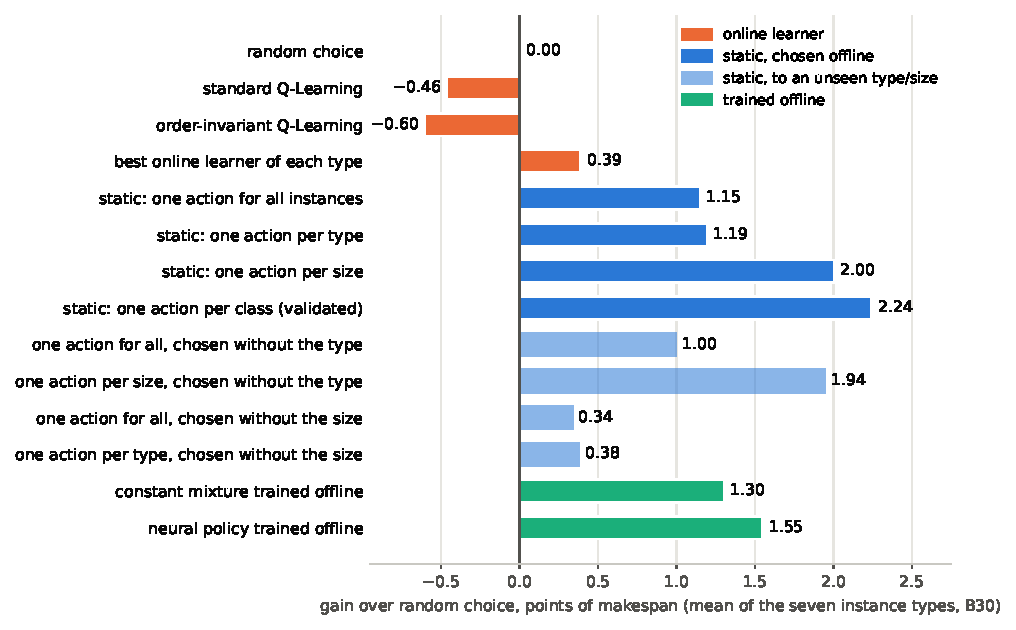
\includegraphics[width=0.92\textwidth]{fig_granularity.pdf}
\caption{The value of offline knowledge by granularity (standard benchmark, B30): gain over random choice, mean of the seven instance types. Orange: online learners; blue: static actions chosen on the tuning instances (hatched: chosen without the type or the size of the instances tested); green: policies trained offline; dotted orange: the optimistic Q-Learning warm-started with an offline prior (and, in blue, the same prior without learning).}
\label{fig:granularity}
\end{figure}

% Auto-generated by analysis/make_table_journal.py
\begin{table}[t]
\caption{The value of offline knowledge by granularity on the standard benchmark: gain over random choice (points of makespan; mean of the seven instance types, $100$ test instances each, $T=1000$, three seeds) of static actions chosen on the tuning instances with decreasing knowledge of the instance, of the online learners and of the policies trained offline. B30 also shows the share of the class-validated gain. Static actions are chosen only on the tuning instances; the ceiling chooses on two test seeds and evaluates on the third.}
\label{tab:granularity}
\centering
{\scriptsize\setlength{\tabcolsep}{5pt}
\begin{tabular}{@{}lrrrr@{}}
\toprule
Policy & B5 & B15 & B30 & B30, share of $G_{tn}$ \\
\midrule
random choice & 0 & 0 & 0 & 0 \\
best online learner of each type & 0.22 & 0.31 & 0.39 & 17\% \\
standard Q-Learning & $-$0.33 & 0.05 & $-$0.46 & $-$21\% \\
order-invariant Q-Learning & $-$0.06 & $-$0.24 & $-$0.60 & $-$27\% \\
static, one action for all instances ($G_0$) & 0.28 & 1.02 & 1.15 & 51\% \\
static, by type ($G_t$) & 0.32 & 0.99 & 1.19 & 53\% \\
static, by size ($G_n$) & 0.57 & 1.30 & 2.00 & 89\% \\
static, by class (type, size): the validated action ($G_{tn}$) & 0.87 & 1.60 & 2.24 & 100\% \\
static, by class, chosen on the test seeds (cross-fitted ceiling) & 0.87 & 1.61 & 2.23 & 99\% \\
$G_0$ chosen without the type of the instance & 0.28 & 1.02 & 1.00 & 45\% \\
$G_n$ chosen without the type of the instance & 0.35 & 1.10 & 1.94 & 87\% \\
$G_0$ chosen without the size of the instance & 0.28 & 1.02 & 0.34 & 15\% \\
$G_t$ chosen without the size of the instance & $-$0.40 & 0.33 & 0.38 & 17\% \\
constant mixture trained offline (nn\_const) & -- & 1.03 & 1.30 & 58\% \\
neural policy trained offline (nn) & -- & 1.07 & 1.55 & 69\% \\
\bottomrule
\end{tabular}}
\end{table}


\paragraph{Where online learning pays, and how to build it (post hoc, then registered)} The unseen-size regime is the one place where an online learner beat an offline static action, at the two extreme sizes ($n=100$ and $n=1000$): at $n=100$ the transferred action \emph{loses} $1.19$ points to random choice while the FRRMAB-style learner is level with it, and at $n=1000$ the optimistic Q-Learning gains $0.83$ against $0.37$. We then built the insurance: the optimistic Q-Learning is warm-started with a prior computed on the tuning instances only (the initial value of an action is its score in $[0,1]$ times the optimism factor of the cold learner). With the prior taken from the other sizes it gains $1.07$ points, against $0.31$ for the cold learner and $0.38$ for the transferred static action. With the prior of the class itself it gains $1.97$ ($88\%$ of the class-validated gain) but never beats the class-validated action. A control with the learning rate set to zero shows what learning adds: without it the transferred prior is worth what the transferred static action is worth ($0.40$ against $0.38$) and the class prior what the validated action is worth ($2.25$ against $2.24$); learning adds $0.67$ points when the prior was transferred (six of seven types) and costs $0.28$ when the prior was exact. The online learner is a \emph{corrector} of offline knowledge: it earns what the prior lacks and pays for what the prior already had. Six of the seven predictions of the warm-start battery held, and all five of its control.

\subsection{A second domain: the iterated local search for the travelling salesman problem}
\label{sec:tsp}
\paragraph{Design and results} To test whether the findings belong to scheduling, we applied the protocol unchanged to an iterated local search for the Euclidean TSP: a tour improved by 2-opt and Or-opt with neighbour lists, a perturbation chosen at each iteration by the selector (a local double-bridge, short random reversals, or the shuffle of a segment; five sizes of each; spaces T5 and T15) and acceptance of a candidate that is not worse. Instances are uniform or clustered points with $n\in\{200,500,1000,2000\}$ (eight classes, $12$ tuning and $50$ test instances each, $T=1000$, three seeds; learners with frozen hyperparameters). The picture of the scheduling hosts repeats (Table~\ref{tab:tsp}). The validated action gains over random choice beyond the margin in all $16$ cells ($0.05$ to $0.90$ points of the tour length) and none of the six online learners beats it beyond the margin in any of the $96$ learner--cell pairs. The standard Q-Learning loses to random choice in every cell ($0.13$ to $0.63$ points) and the lock-in reproduces: it puts $61\%$ of its choices in T15 on the action listed first and evaluates $0.64$ times as many moves as random choice; the permuted version gains in no cell and differs from it beyond the margin in $15$ of $16$ cells. Thompson sampling gains in $7$ of $16$ cells (up to $0.38$ points), but the best online learner of a cell recovers at most half of the validated gain in $12$ of the $16$. All ten predictions held. On $37$ instances of the TSPLIB~\cite{Reinelt1991} (static actions chosen only on the synthetic tuning instances), the static action gains beyond the margin in both spaces ($0.53$ and $0.56$ points; one action for all gains $0.53$ and $0.68$), no online learner beats it, the best, Thompson sampling, recovers $23\%$ and $43\%$ of its gain, and the static action ends on average $1.21\%$ above the optimal tour in T15 (random choice: $1.79\%$); all nine predictions held.

\paragraph{The hierarchy of knowledge is not universal} In the TSP the finest knowledge adds nothing: one action chosen for all instances gains $0.54$ points in T15, more than the class-validated action ($0.50$, chosen on $12$ tuning instances per class), and the action chosen without the size of the tested instances gains beyond the margin at all four sizes. The importance of the size found with the scheduling benchmark is a property of that host, whose best action changes with $n$; what carries over is that a static action chosen offline, at whatever granularity, beats every online learner.

% Auto-generated by analysis/make_table_journal.py
\begin{table}[t]
\caption{A second domain: the iterated local search for the Euclidean TSP. Gain over random choice (percentage points of the tour length, positive = better; $50$ test instances per class, $T=1000$, three seeds) of the validated action (val), the standard Q-Learning (ql), Q-Learning with the actions permuted in each run (ql\_perm), UCB1, the policy gradient (pg), the ALNS roulette (alns), Thompson sampling (ts) and the optimistic Q-Learning (qo). T5: five perturbation sizes; T15: three perturbations $\times$ five sizes. Bold: gain confirmed (Holm over the eight classes of each method and space) and not equivalent to zero at the margin $\pm0.05$. No online learner beats the validated action beyond the margin in any of the $96$ learner--cell pairs.}
\label{tab:tsp}
\centering
{\scriptsize\setlength{\tabcolsep}{4pt}
\begin{tabular}{@{}llrrrrrrrr@{}}
\toprule
Space & Class & val & ql & ql\_perm & ucb & pg & alns & ts & qo \\
\midrule
T5 & clustered $n=200$ & \textbf{0.12} & $-$0.15 & $-$0.05 & 0.03 & $-$0.02 & 0.04 & 0.05 & 0.02 \\
T5 & clustered $n=500$ & \textbf{0.59} & $-$0.46 & 0.00 & 0.17 & 0.22 & 0.04 & 0.27 & 0.23 \\
T5 & clustered $n=1000$ & \textbf{0.51} & $-$0.63 & $-$0.17 & $-$0.12 & $-$0.08 & $-$0.14 & \textbf{0.24} & 0.00 \\
T5 & clustered $n=2000$ & \textbf{0.35} & $-$0.53 & $-$0.02 & 0.06 & 0.02 & $-$0.07 & \textbf{0.38} & \textbf{0.20} \\
T5 & uniform $n=200$ & \textbf{0.08} & $-$0.34 & $-$0.11 & $-$0.05 & $-$0.09 & $-$0.12 & 0.01 & $-$0.05 \\
T5 & uniform $n=500$ & \textbf{0.29} & $-$0.38 & $-$0.14 & $-$0.02 & $-$0.01 & $-$0.10 & 0.08 & 0.04 \\
T5 & uniform $n=1000$ & \textbf{0.49} & $-$0.40 & $-$0.07 & 0.05 & \textbf{0.06} & $-$0.05 & \textbf{0.25} & \textbf{0.11} \\
T5 & uniform $n=2000$ & \textbf{0.55} & $-$0.42 & 0.03 & \textbf{0.07} & 0.01 & $-$0.02 & \textbf{0.30} & \textbf{0.13} \\
T5 & mean & 0.37 & $-$0.41 & $-$0.07 & 0.02 & 0.01 & $-$0.05 & 0.20 & 0.08 \\
\midrule
T15 & clustered $n=200$ & \textbf{0.05} & $-$0.13 & $-$0.07 & $-$0.01 & $-$0.03 & $-$0.08 & $-$0.01 & 0.00 \\
T15 & clustered $n=500$ & \textbf{0.36} & $-$0.37 & $-$0.13 & 0.02 & 0.10 & $-$0.13 & 0.16 & 0.14 \\
T15 & clustered $n=1000$ & \textbf{0.77} & $-$0.53 & $-$0.16 & 0.07 & $-$0.01 & $-$0.20 & 0.11 & 0.05 \\
T15 & clustered $n=2000$ & \textbf{0.90} & $-$0.48 & $-$0.09 & 0.00 & $-$0.04 & $-$0.15 & \textbf{0.28} & \textbf{0.09} \\
T15 & uniform $n=200$ & \textbf{0.09} & $-$0.15 & $-$0.05 & 0.04 & 0.03 & 0.01 & 0.06 & 0.03 \\
T15 & uniform $n=500$ & \textbf{0.39} & $-$0.32 & $-$0.12 & 0.02 & 0.02 & $-$0.13 & 0.04 & 0.00 \\
T15 & uniform $n=1000$ & \textbf{0.67} & $-$0.29 & $-$0.10 & 0.02 & 0.06 & $-$0.13 & \textbf{0.18} & 0.08 \\
T15 & uniform $n=2000$ & \textbf{0.80} & $-$0.34 & 0.02 & 0.05 & 0.02 & $-$0.08 & \textbf{0.24} & 0.07 \\
T15 & mean & 0.50 & $-$0.33 & $-$0.09 & 0.03 & 0.02 & $-$0.11 & 0.13 & 0.06 \\
\bottomrule
\end{tabular}}
\end{table}


% Auto-generated by analysis/make_table_journal.py
\begin{table}[t]
\caption{The TSP host on $37$ published TSPLIB instances ($200\le n\le2103$, EUC\_2D; $T=1000$, three seeds): gain over random choice (percentage points of the tour length, positive = better; unit: the instance) and mean gap to the optimal tour length of the TSPLIB (\%). The static actions were chosen on the synthetic tuning instances of Section~\ref{sec:tsp}, not on TSPLIB instances. Bold: gain over random choice confirmed (Holm over the nine methods of each space) and not equivalent to zero at the margin $\pm0.05$. No online learner beats the static action of the nearest size beyond the margin.}
\label{tab:tsplib}
\centering
{\scriptsize\setlength{\tabcolsep}{5pt}
\begin{tabular}{@{}lrrrr@{}}
\toprule
 & \multicolumn{2}{c}{T5} & \multicolumn{2}{c}{T15} \\
\cmidrule(lr){2-3}\cmidrule(lr){4-5}
Method & gain & gap & gain & gap \\
\midrule
random choice & 0 & 1.93 & 0 & 1.79 \\
static, chosen on synthetic instances of the nearest size & \textbf{0.53} & 1.38 & \textbf{0.56} & 1.21 \\
static, one action chosen on synthetic instances & \textbf{0.53} & 1.38 & \textbf{0.68} & 1.08 \\
standard Q-Learning & $-$0.61 & 2.56 & $-$0.34 & 2.14 \\
Q-Learning with permuted actions & $-$0.15 & 2.08 & $-$0.19 & 1.98 \\
UCB1 & 0.04 & 1.88 & 0.05 & 1.73 \\
policy gradient & $-$0.04 & 1.97 & 0.03 & 1.76 \\
ALNS roulette & $-$0.02 & 1.95 & $-$0.11 & 1.90 \\
Thompson sampling & 0.12 & 1.80 & \textbf{0.24} & 1.54 \\
optimistic Q-Learning & 0.02 & 1.91 & 0.07 & 1.72 \\
\bottomrule
\end{tabular}}
\end{table}


\paragraph{The warm start in the TSP} The warm-start experiment repeats on the TSP host (Entries 274 and 275; nine and seven predictions recorded beforehand, six of each held). Because the rankings of the actions of the eight classes almost coincide (Spearman correlation at least $0.92$), a prior taken from the other sizes is nearly exact, so we also gave the learner a deliberately wrong prior, the reversed ranking of the class (Table~\ref{tab:tspwarm}). With the prior of the class the warm-started learner gains $0.49$ points in T15, level with the class-validated action ($0.50$) and eight times the cold learner ($0.06$); the same prior without learning gains $0.50$. Learning therefore costs little where the prior is nearly exact ($0.005$ and $0.046$ points; the cost of at least $0.10$ points that we predicted did not materialise) and adds $0.72$ points against the reversed prior, beyond the margin in all eight classes, although the correction is far from complete ($-1.32$ against $-2.03$ for the frozen prior). On the $37$ TSPLIB instances, with the prior taken from synthetic instances only, the warm-started learner gains $0.56$ points, against $0.07$ for the cold learner and $0.56$ for the static action of the nearest size, and the effect of learning follows the quality of the prior by size band: in the $15$ small instances, where that static action does not gain ($-0.02$), it gains $0.21$ points, $0.07$ more than the same prior without learning, whereas in the $22$ medium and large instances, where the static action gains $0.96$, learning costs $0.16$ points. The frozen variants evaluate $1.38$ to $1.59$ times as many moves as the learner, so these comparisons are at equal iterations, not at equal CPU time.

% Auto-generated by analysis/make_table_journal.py
\begin{table}[t]
\caption{The optimistic Q-Learning warm-started with an offline prior in the TSP host: gain over random choice (percentage points of the tour length, positive = better). Panel A: the eight synthetic classes ($50$ test instances each, $T=1000$, three seeds; mean of the eight class gains); the prior of the class (full), of the other sizes of the same type (loso) or the reversed ranking of the class (rev), with learning (warm) and without (frozen, learning rate zero); help/cost: classes in which learning gains/loses beyond the margin $\pm0.05$ (Holm over the eight classes); static: the validated action (full) or the action chosen without the size (loso). Panel B: the $37$ TSPLIB instances (T15), with the prior of the synthetic size nearest to the instance (synn) or of all synthetic classes (syn0); Gn and G0 are the static actions of Table~\ref{tab:tsplib}; bands: small ($n<500$), medium and large.}
\label{tab:tspwarm}
\centering
{\scriptsize\setlength{\tabcolsep}{3pt}
\resizebox{\textwidth}{!}{\begin{tabular}{@{}llrrrrrrr@{}}
\toprule
\multicolumn{9}{@{}l}{\emph{A. Synthetic TSP}} \\
Space & prior & warm & frozen & warm$-$frozen & help & cost & cold qo & static \\
\midrule
T15 & full & 0.49 & 0.50 & $-$0.01 & 0 & 1 & 0.06 & 0.50 \\
T15 & loso & 0.48 & 0.53 & $-$0.05 & 0 & 1 & 0.06 & 0.54 \\
T15 & rev & $-$1.32 & $-$2.03 & 0.72 & 8 & 0 & 0.06 & -- \\
\midrule
T5 & full & 0.34 & 0.36 & $-$0.02 & 1 & 0 & 0.08 & 0.37 \\
T5 & loso & 0.37 & 0.38 & $-$0.02 & 0 & 1 & 0.08 & 0.42 \\
T5 & rev & $-$1.08 & $-$1.54 & 0.46 & 8 & 0 & 0.08 & -- \\
\midrule
\multicolumn{9}{@{}l}{\emph{B. TSPLIB (T15)}} \\
Band & $n$ & warm synn & frozen synn & warm syn0 & frozen syn0 & cold qo & Gn & G0 \\
\midrule
small & 15 & 0.21 & 0.14 & 0.31 & 0.19 & 0.16 & $-$0.02 & 0.28 \\
medium and large & 22 & 0.80 & 0.96 & 0.77 & 1.01 & 0.01 & 0.96 & 0.96 \\
all & 37 & 0.56 & 0.63 & 0.58 & 0.68 & 0.07 & 0.56 & 0.68 \\
\bottomrule
\end{tabular}}}
\end{table}


\section{Discussion}
\label{sec:discussion}
\paragraph{What the evidence says} The gains that learning-guided search reports are mostly \emph{structure} (destruction--reconstruction), \emph{budget} and \emph{tuning}. The learner's own contribution, the decision effect, is bounded by one quantity, the headroom of the best fixed action net of run-to-run noise: below about $0.05$ points the online learner never gained beyond the equivalence margin in any cell outside those that set the threshold, and above it none was shown to once the order of the actions is randomised (the standard learner repeats the action listed first, and an order-invariant Q-Learning gains beyond the margin in none of $85$ cells). What headroom rewards is knowledge acquired \emph{before} the run: a validated action, a selector trained offline (about four fifths of the one-seed oracle gain on $P||\Cmax$, $60$--$73\%$ on unrelated machines) or a neural policy (two thirds of the validated gain; $60\%$ out of that $67\%$ is already a constant mixture). How much offline knowledge is needed depends on the host: on the standard $R||\Cmax$ benchmark one action for all instances already gains $51\%$ of the class-validated gain and the size of the instance supplies $89\%$ of it, whereas in the TSP no finer knowledge adds anything. The one regime in which an online learner beat an offline static action is a transferred action applied to an unseen extreme size; there the learner is an insurance, best built as a correction of the offline prior: warm-started with it, the optimistic Q-Learning gains $0.67$ points over the same prior without learning when the prior was transferred and loses $0.28$ when it was exact. Where actions are complementary (the genetic algorithm, the ILS operators) the static competitor must be a \emph{mixture}; the claim that a validated static configuration is never beaten beyond the margin concerns the best of a single action or a validated mixture.

\paragraph{Why the usual comparison misleads} Comparing a learning-guided metaheuristic with a non-learning one changes at least four things at once: the search structure, the number of iterations or the CPU time, the tuning effort of each side, and the information the learner receives. The protocol varies one at a time: the learning-guided IG appeared to owe its advantage over the ILS to the learner when it belongs to the destruction--reconstruction mechanism; at equal CPU time the learner appeared responsible for a gain that belongs to choosing cheaper actions; and a one-seed oracle appeared to show room for improvement that was mostly noise. In the literature we audited, $22$ of $23$ papers report a benefit of the learned component, $10$ include a random-selection control, $6$ compare at a common time limit and $3$ a static configuration; the audit counts which controls were reported, not whether the claims are true.

\paragraph{A checklist for a claim that a learned selector helps}
\begin{enumerate}
\item Report a \textbf{random control over the same actions at the same budget}, with the same code path as the learner.
\item At equal CPU time, \textbf{calibrate the cost ratio} $K$ on separate instances, report it for every arm, and split the gain into a decision effect and a cost effect.
\item \textbf{Validate a static action (or a mixture) offline} on instances disjoint from the test set, with the same effort the learner's tuning received; add a configurator and a published AOS design where they apply.
\item Estimate the headroom \textbf{with cross-fitting}, and report the one-seed value (an upper bound) and the cross-fitted value (a lower bound).
\item Include a \textbf{positive control} and an \textbf{equivalence margin}, so that ``no effect'' is a finding and not a failure to reject.
\item \textbf{Record hypotheses, decision rules and predictions before running}, with hashes of the code and frozen inputs, and control the error rate within each family of tests.
\item Report the learner's \textbf{sensitivity to the order of the actions}: the share of choices on the action listed first, and the result with the actions permuted (or ties broken at random).
\item State \textbf{what the static competitor knows} and test its transfer to an instance type or size it was not tuned for; an online learner warm-started with the offline prior can be worth its cost exactly where the transferred action fails, and costs something where the prior is exact.
\end{enumerate}

\paragraph{What the registered predictions showed} \npredheld{} of \npredtotal{} point predictions held in \nbatteries{} batteries. The misses (cost ratios, the classic AOS methods, the flowshop, warm-started Q-Learning, finer times) led to the headroom rule and to cross-fitting. The headline pairs keep their significance under Pratt's treatment of ties and a permutation test, $1{,}606$ of the $1{,}674$ confirmed tests survive a global Benjamini--Yekutieli control over the $3{,}578$ tests of all registered batteries (each extension of the control was itself registered, three predictions of three).

\section{Limitations}
\label{sec:limitations}
\begin{enumerate}[label=(\roman*)]
\item \emph{Equal CPU time} depends on $K$, measured on separate instances in sequence and reported for every arm; a learner whose actions are cheap can win on cost alone, which is why the decomposition is part of the protocol.
\item \emph{Practical significance.} Gains are in points of the makespan, and the margin is a choice. The hosts are not far from the best known values: on the standard benchmark the validated action ends $4.89\%$ above the best known solutions at $T=1000$ and $2.69\%$ at $T=10^4$, and in the TSP $1.21\%$ above the optimum of the TSPLIB instances (T15).
\item \emph{Registration and multiplicity.} Each battery has its own Holm family; the headroom rule began as an exploratory reading. The pre-specification is a dated, hash-stamped diary under version control, not a public registry.
\item \emph{Scope.} The evidence is for $P||\Cmax$, $R||\Cmax$, a permutation flowshop, one genetic algorithm and one TSP local search, with tabular and bandit learners, a DQN on joint actions and two published AOS designs. Deep policy gradients that learn during the run and portfolios of hundreds of operators are outside the evidence, and the neural policy is one architecture trained on one host.
\item \emph{Implementation dependence.} A conclusion about ``Q-Learning'' is a conclusion about an implementation (initial values, tie rule, reward sign); we did not rerun UCB1, the policy gradient and the roulette with permuted actions, and the irace-tuned Q-Learning keeps the standard tie rule.
\item \emph{Offline knowledge.} The map by granularity ran on one scheduling benchmark and the TSP; the unseen-size reading is post hoc and rests on the two extreme sizes of four; the warm-start result is for one learner and one prior construction.
\item \emph{Horizons} up to $T=10^5$ were studied on two hosts and $T=10^4$ on the standard benchmark in the richest space only; a learner that needs a longer horizon than the headroom lasts for is not excluded in general.
\item \emph{Selector cost.} Training costs of the offline selector and of the neural policy ($115{,}200$ and $138{,}240$ IG runs, eight to fourteen times the tuning of the validated action) are not charged to them.
\item \emph{Review status.} The manuscript has not been externally reviewed; simulated blind reviews guided the revisions but are not a substitute.
\end{enumerate}

\section{Conclusion}
\label{sec:conclusion}
A learned operator selector is not what explains the advantage of an IG over ILS for identical parallel machines: that belongs to destruction--reconstruction, and the share of a local search's gain that is only budget ($93\%$, $30\%$ or $28\%$ by implementation) makes the CPU cost ratio a result to report. The oracle headroom net of run-to-run noise bounds what a validated action or an offline policy can capture, and online Q-Learning did not pay at these budgets: the gains first attributed to it came from the standard implementation repeating the action listed first, and an order-invariant version gains beyond the margin in none of $85$ cells. A validated static configuration was never worse than an online learner beyond the margin on any host, on published instance families, on the standard benchmark and at a ten times longer horizon (at equal CPU time on the standard benchmark it lost two of $49$ pairs). What pays is offline knowledge: one action chosen offline for all instances beats every online learner, the size of the instance carries nine tenths of what class-level knowledge gives, and an online learner is worth having as a corrector of that knowledge where it does not cover the instance (a size never tuned for): warm-started with the offline prior it recovers $48\%$ of the class-level gain there, against $17\%$ for the transferred static action, and without a prior it recovers $14\%$. The same asymmetry appears in the TSP, an iterated local search for a different kind of problem: learning helps against a wrong prior and costs little against a nearly exact one.

For the practitioner the message is a procedure more than a verdict: before crediting a learned component, compare it with random choice at the same budget, with a static choice validated offline and with a configurator, permute the order of the actions to see whether the learner is learning or repeating the first item of its list, and ask whether the headroom is large enough for any online method to find. For the researcher it is a set of estimators with stated and checked properties and a registry of $\npredtotal$ pre-recorded predictions, whose misses are listed and changed the analysis.

\paragraph{Data and code availability} Code, instances, results, the research diary with the pre-registered hypotheses and md5 hashes, the protocol library and the scripts that recompute every number are at \url{https://github.com/CarlosAraujo7/pmsp}. \todonote{funding statement: CAPES/FUNCAP/CNPq to confirm; anonymised repository link for review}


\bibliographystyle{elsarticle-harv}
\bibliography{refs}
\end{document}
